\chapter{Learning Paradigms}\label{ch:para}

Throughout this thesis, we assume to be given data $\Inp_n\subset\Inp\subset \R^d$ consisting of $n$ data points. We consider task of \emph{learning} a function $f:\tilde{\Inp}\to \Oup$ from the given data, where the two most important cases for us are
%
\begin{itemize}
\item \textbf{classification}: $\net$ assigns a label to each $x\in \tilde\Inp$ out of a total of $C\in\N$ possible classes, i.e. $\Oup=\{1,\ldots,C\}$. In some architectures the last layer of the neural network is given as a vector $\oup\in\R^C$. Typically, this vector is a probability vector, i.e. 
%
\begin{align*}
y\in \Delta^C := \left\{z\in[0,1]^d: \sum_{i=1}^C z_i = 1\right\}.
\end{align*}
%
This can be enforced via the softmax function \cite{bridle1990probabilistic} $\operatorname{soft max}:\R^d\to\R^d$
%
\begin{align*}
\operatorname{soft max}(z)_i := \frac{\exp(z_i)}{\sum_{j=1}^C \exp(z_j)} 	
\end{align*}
%
which was actually introduced by Boltzman in \cite{boltzmann1868studien}. This allows the interpretation that the $i$th entry of $\net_\param(\inp)\in\Delta^C$ models the probability that $\inp$ belongs to class $i$. In order to obtain a label one can simply choose the maximum entry, $\argmax_{i=1,\ldots,C} \net_\param(\inp)_i$.
%
\item \textbf{image denoising}: $\net$ outputs a denoised version of an input image. Here we have $\Inp = \Oup=\R^{K\times N\times M}$, where
%
\begin{itemize}
\item $K\in\N$ is the number of color channels,
\item $N,M$ denote the width and height of the image.
\end{itemize}
\end{itemize}
%
The set $\tilde{\Inp}\subset\R^d$ is usually either the set of data points $\Inp_n$ or the whole space $\Inp$. The learning paradigms we consider in this thesis, differ by their usage of labeled data. We review the concepts in the following.
%
\section{Unsupervised Learning}
\begin{wrapfigure}{r}{.5\textwidth}
\centering
\includegraphics[width=.5\textwidth]{atelier/paradigms/UL.pdf}
\end{wrapfigure}

In this case we are not given any labeled data. In our context the most important application is data clustering. Other tasks involve dimensionality reduction or density estimation, see \cite{subramanya2014graph}. The clustering task consists of grouping data based on some similarity criterion. In this sense, clustering can also be interpreted as classification, i.e., the desired function is a mapping $\net:\tilde{\Inp}\to \{1,\ldots, C\}$ where $C\in\N$ denotes the number of clusters. Typically, one wants to obtain a clustering of the given data set, i.e., $\tilde\Inp = \Inp_n$. We list some of the typical clustering methods below:
%
\begin{itemize}
\item K-means algorithm \cite{steinhaus1956division},
\item Expectation Maximization  \cite{dempster1977maximum},
\item Cheeger cuts \cite{GarcSlep15, szlam2009total, trillos2016consistency, garcia2022graph},
\item spectral clustering \cite{trillos2018variational, trillos2021geometric, hoffmann2022spectral}.
\end{itemize}
%
%
Unsupervised learning is not the main focus of this present work. However, we note that especially the concepts developed in \cite{GarcSlep15} for Cheeger cuts are crucial for the continuum limit framework in \cref{sec:GConv}.

\section{Supervised Learning}\label{sec:PSL}
\begin{wrapfigure}{r}{.5\textwidth}
\centering
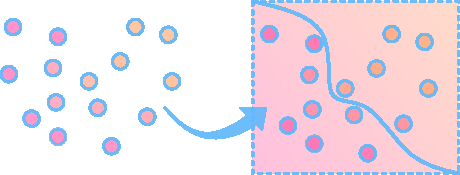
\includegraphics[width=.5\textwidth]{atelier/paradigms/SL.pdf}
\end{wrapfigure}
%
In this setting, each data point $x\in\Inp_n$ is labeled, via a given function $g:\Inp_n\to\Oup$ such that we have a finite training set $\mathcal{T} = \{(x,g(x)): x\in\Inp_n\}$. The task is then to infer a function defined on the underlying space, i.e. $\net:\Inp \to\Oup$, i.e. we want to assign a label to unseen $x\in\Inp$ that are not necessarily part of the given data. Often, one models the problem via a joint probability function $P_{\Inp,\Oup}$ and assumes that the training data are i.i.d. w.r.t. $P_{\Inp,\Oup}$. In this interpretation, a neural network can aim to model the conditional $P(y|x)$ for an input $\inp\in\Inp$ and output $\oup\in\Oup$.


In order to \emph{learn} the function $\net$ from the given data, one needs to choose a parameterized class of functions $\mathcal{U}$, where typically each element can be describe by a finite number of parameters. Among others, common methods or parametrizations include
%
\begin{itemize}
\item Support vector machines \cite{cortes1995support, scholkopf2005support},
\item decision Trees \cite{morgan1963problems, Brei},
\item neural networks \cite{Turing,rosenblatt1958perceptron, minsky1969introduction}.
\end{itemize}
%
In \cref{sec:SL} we exclusively focus on supervised learning algorithms employing neural networks. We refer to \cite{SCHMIDHUBER201585} for an exhaustive historical overview. The concrete setting and learning framework is given in \cref{ch:SL}.
%
%
%
\section{Semi-Supervised Learning}\label{sec:PSSL}
\begin{wrapfigure}{r}{.5\textwidth}
\centering
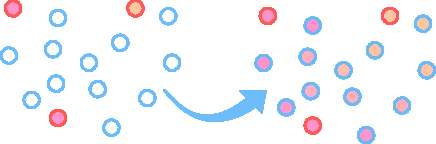
\includegraphics[width=.5\textwidth]{atelier/paradigms/SSL.pdf}
\end{wrapfigure}
%
In the semi-supervised setting we assume that only a fraction of the data $\Inp_n$ is labeled, i.e., we are given a a function $g:\conset_n\to\Oup$ where $\conset_n\subset\Inp_n$ is the set of labeled data. Typically the labeled data constitutes only a small fraction of all available points, i.e. $\abs{\conset_n}<<\abs{\Inp_n}$. In this thesis we restrict ourselves to the \emph{transductive setting}, i.e. we want to infer a function acting only on the data $\net: \Inp_n\to \Oup$. This is opposed to the inductive setting, where $\net$ also classifies unseen points $x\in\Inp$, \cite{zhu2005semi}. Common algorithms and methods include
%
\begin{itemize}
\item expectation maximization and mixture models \cite{dempster1977maximum,cozman2003semi},
\item self-training and co-training \cite{blum1998combining},
\item graph-based learning \cite{zhu2005semi}.
\end{itemize}
%
%
Mostly, we consider the extension task with $\Oup$ being chosen as $\R$. In application this can be seen as a binary classification task, where for $o\in\conset_n$ we have $g(o)=1$ if $o$ belongs to a some class and $g(o)=0$ otherwise. The function $f:\Inp_n\to\R$ then determines the probability that any vertex $x\in X_n$ belongs o this class, where we can binarize the output afterwards via some thresholding, e.g.,
%
\begin{align*}
x \text{ belongs to the class } \Leftrightarrow f(x) > 0.5
\end{align*}
%
This methodology can be extended to classification tasks beyond the binary case, via the so-called one-vs-all technique \cite{zhu2003semi}. Given a classification problem with $C\in\N$ possible classes, we assume that the labeling function $g:\conset_n\to \Delta^C$ outputs one-hot vectors, i.e. $g(o)_c =1$ if $o$ belongs to class $c$ and $g(o)_c=0$ otherwise, for every $c = 1,\ldots, C$. We then perform the binary classification problem \enquote{$x$ belongs to class $c$} for every $c=1,\ldots,C$, by considering the extension task of 
%
\begin{align*}
g_c:\conset_n\to\R\qquad g_c(o) = g(o)_c,
\end{align*}
%
which yields a function $f_c(o)$. The final output can then either obtained by taking the argmax, i.e. $f:\Inp_n\to\{1,\ldots, C\}$ 
%
\begin{align*}
f(x) := \argmax_{c=1,\ldots, C} f_c(x)
\end{align*}
%
or by applying a softmax to obtain a probability vector, i.e. $f:\Inp_n\to\Delta^C$ 
%
\begin{align*}
f(x) := \operatorname{soft max}\left(f_1(x), \ldots, f_c(x)\right).
\end{align*}
%
In \cref{ch:SSL} we focus on graph-based learning algorithms, however we refer to \cite{zhu2005semi} for a overview of semi-supervised learning algorithms. 
